%%%%%%%%%%%%%%%%%%%%%%%%%%%%%%%%%%%%%%%%%
% Ay 190 - Final Project
% Written by Chatarin Wong-u-railertkun
%%%%%%%%%%%%%%%%%%%%%%%%%%%%%%%%%%%%%%%%%

%----------------------------------------------------------------------------------------
%	PACKAGES AND OTHER DOCUMENT CONFIGURATIONS
%----------------------------------------------------------------------------------------

\documentclass[11pt,letterpaper]{article}

% Load some basic packages that are useful to have
% and that should be part of any LaTeX installation.
%

\usepackage{graphicx}     % be able to include figures

\usepackage{xcolor}         % get nice colors

% change default font to Palatino (looks nicer!)
\usepackage[latin1]{inputenc}
\usepackage{mathpazo}
\usepackage[T1]{fontenc}

% load some useful math symbols/fonts
\usepackage{latexsym,amsfonts,amsmath,amssymb}
\usepackage{subcaption}

% comfort package to easily set margins
\usepackage[top=1in, bottom=1in, left=1in, right=1in]{geometry}

% control some spacings
%
% spacing after a paragraph
\setlength{\parskip}{.15cm}
% indentation at the top of a new paragraph
\setlength{\parindent}{0.0cm}

\usepackage{courier}


%----------------------------------------------------------------------------------------
%	TITLE
%----------------------------------------------------------------------------------------

\begin{document}

\begin{center}
\Large
Ay190 -- Final Project: Orbital Integrations \\
Chatarin (Mee) Wong-u-railertkun \\
Date: \today
\end{center}

\section{Two-Body Problem: Accumulated Truncation Error}

\subsection{Runge-Kutta vs Leap Frog}

We shall explore the pros and cons of two numerical integrators: RK4 and Leapfrog.

\subsubsection{RK4}
From lecture note, the Runge-Kutta Integrator 4 are defined as, 

\begin{align*}
k_1 &= hf(x_n,y_n), \\
k_2 &= hf(x_n+\frac{h}{2},y_n+\frac{1}{2}k_1), \\
k_3 &= hf(x_n+h, y_n-k_1+2k_2), \\
y_{n+1} &= y_n + \frac{1}{6}(k_1+4k_2+k_3)+O(h^4)
\end{align*}

\subsubsection{Leapfrog}
Leapfrog integration involves calculating velocity at half step. However, the position and velocity at each step is

\begin{align*}
x_{n+1} &= x_n + v_n \Delta t + \frac{1}{2} a_n \Delta t^2, \\
v_{n+1} &= v_n + \frac{1}{2} (a_n + a_{n+1}) \Delta t
\end{align*}	

The RK4 method is not \emph{symplectic} since the position and velocity of the next step based solely on data at current step. On the other hand, for leapfrog method, to calculate velocity at the next step, we have to use position at the next step to calculate acceleration at the next step.

Simulate a two-body system: Sun-Earth. Put Earth in a circular orbit around the sun at 1 AU. Using both RK4 and leapfrog method to simulate the orbit of the Earth around the Sun. Because the RK4 method is not \emph{symplectic}, energy of the system is not conserved. Figure \ref{fig:AddedError} shows the error in total energy, $\left | \frac{\Delta E}{E} \right |$ of these two methods overtime. Even though the error of the leapfrog method oscillates, it returns to its original value. On the other hand, error of the RK4 keeps accumulating.

\begin{figure}[h!]
	\centering
	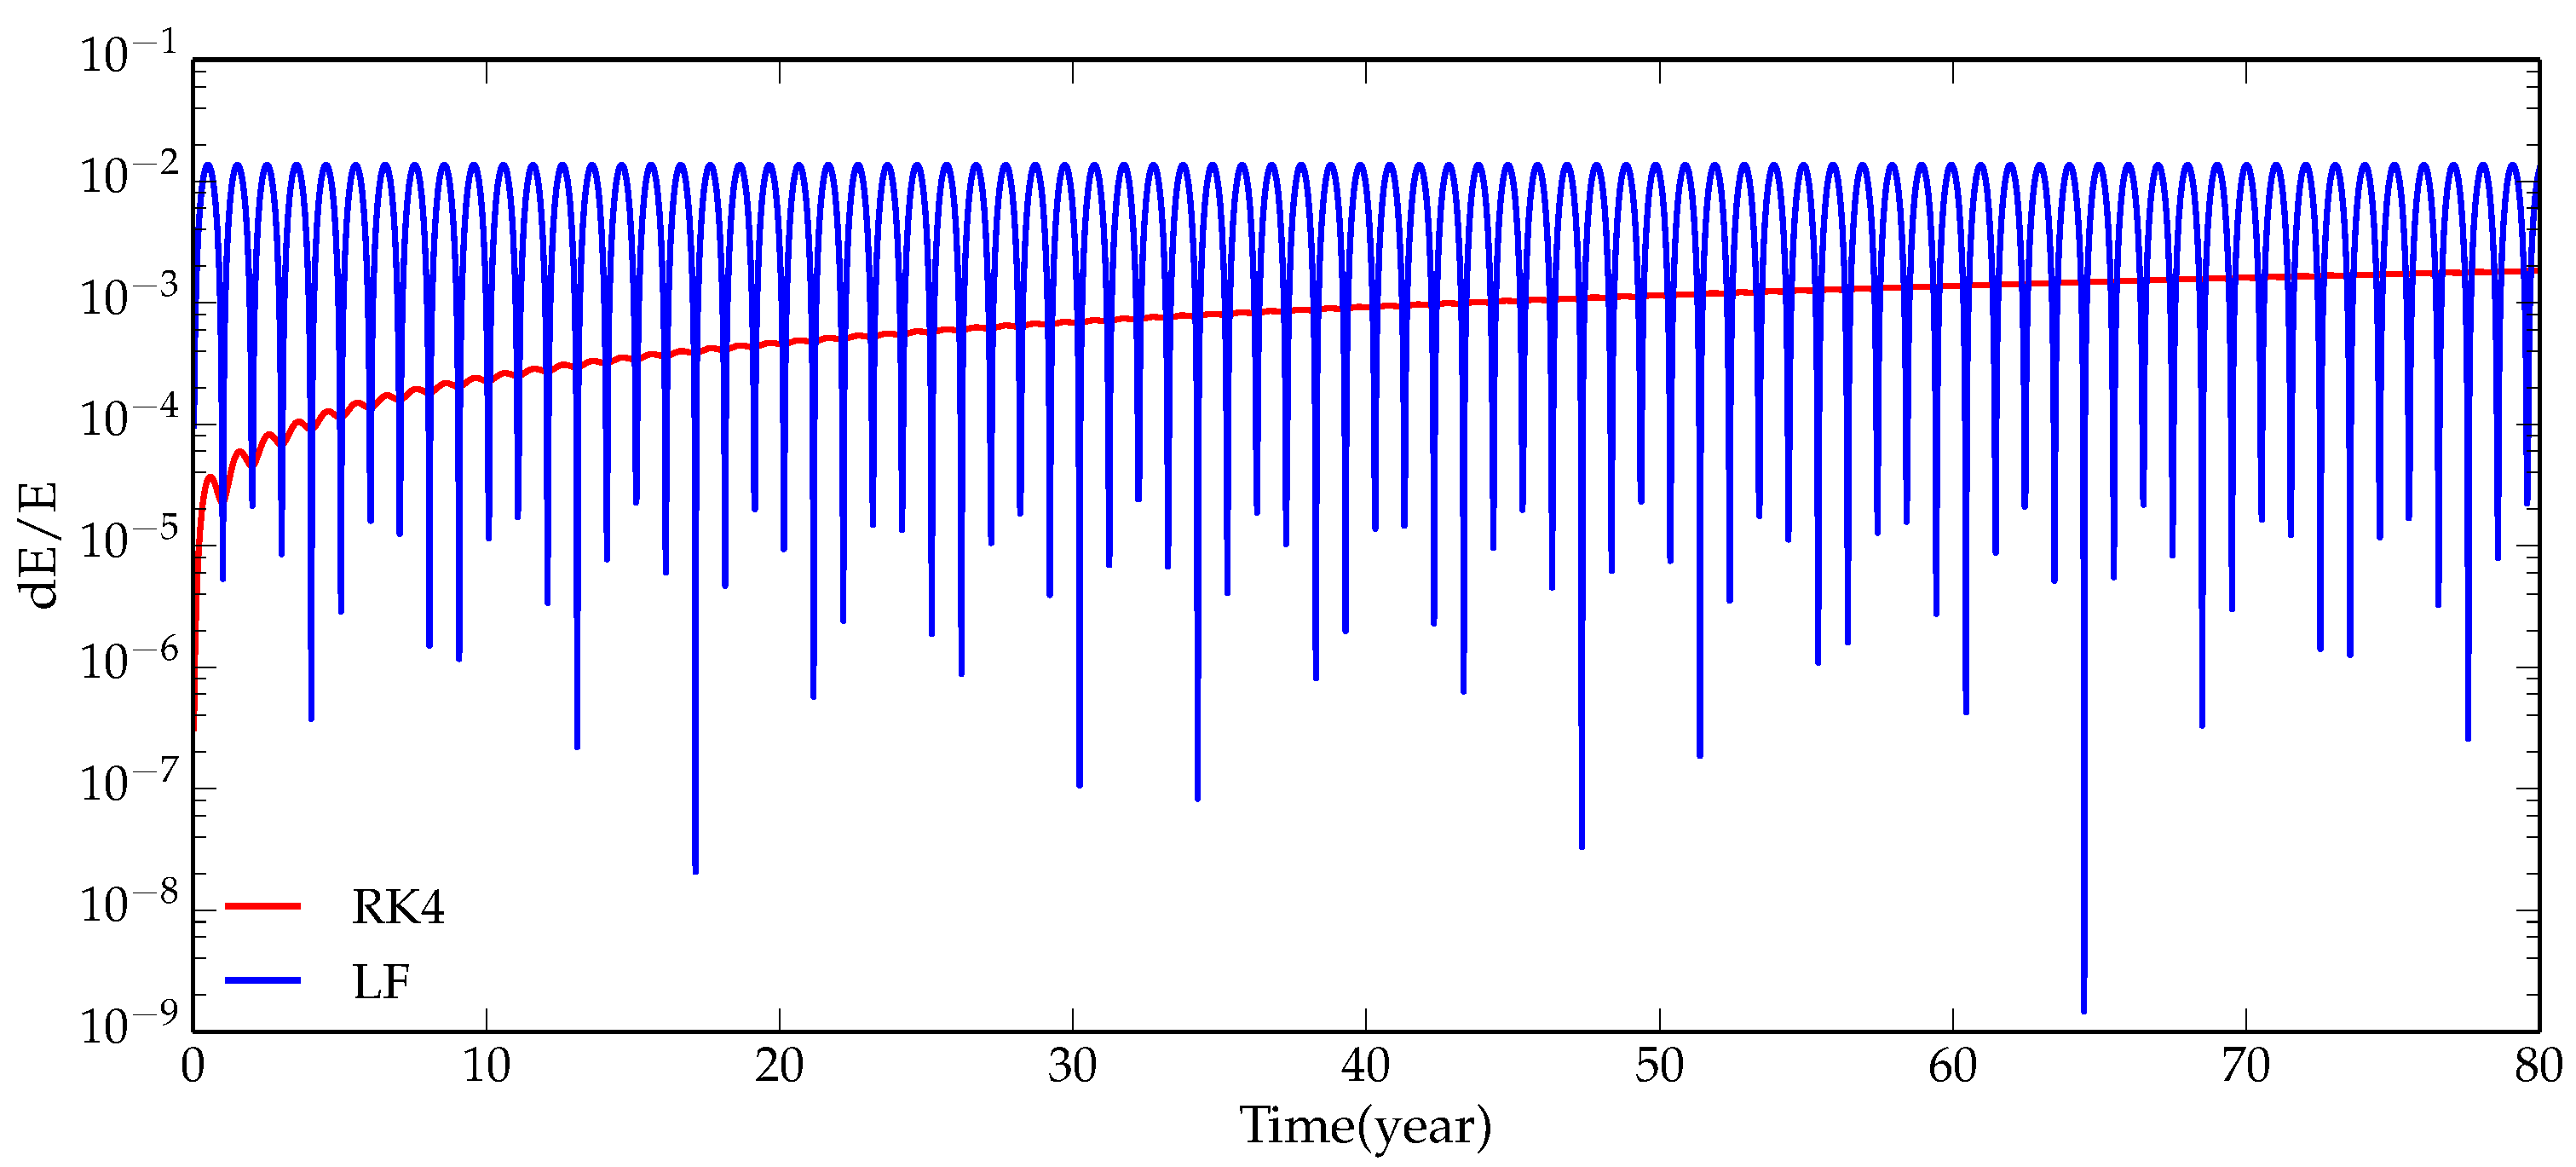
\includegraphics[height = 0.3\textheight]{AddedError}
	\caption{Error of RK4 vs. Leapfrog: Even though the error of leapfrog method oscillates, it returns to the same value, i.e. the error is not increasing. On the other hand, error of RK4 method, also oscillating, continuously increases over time.}
	\label{fig:AddedError}
\end{figure}

\subsection{Resolution}

\begin{figure}[h!]
	\centering
	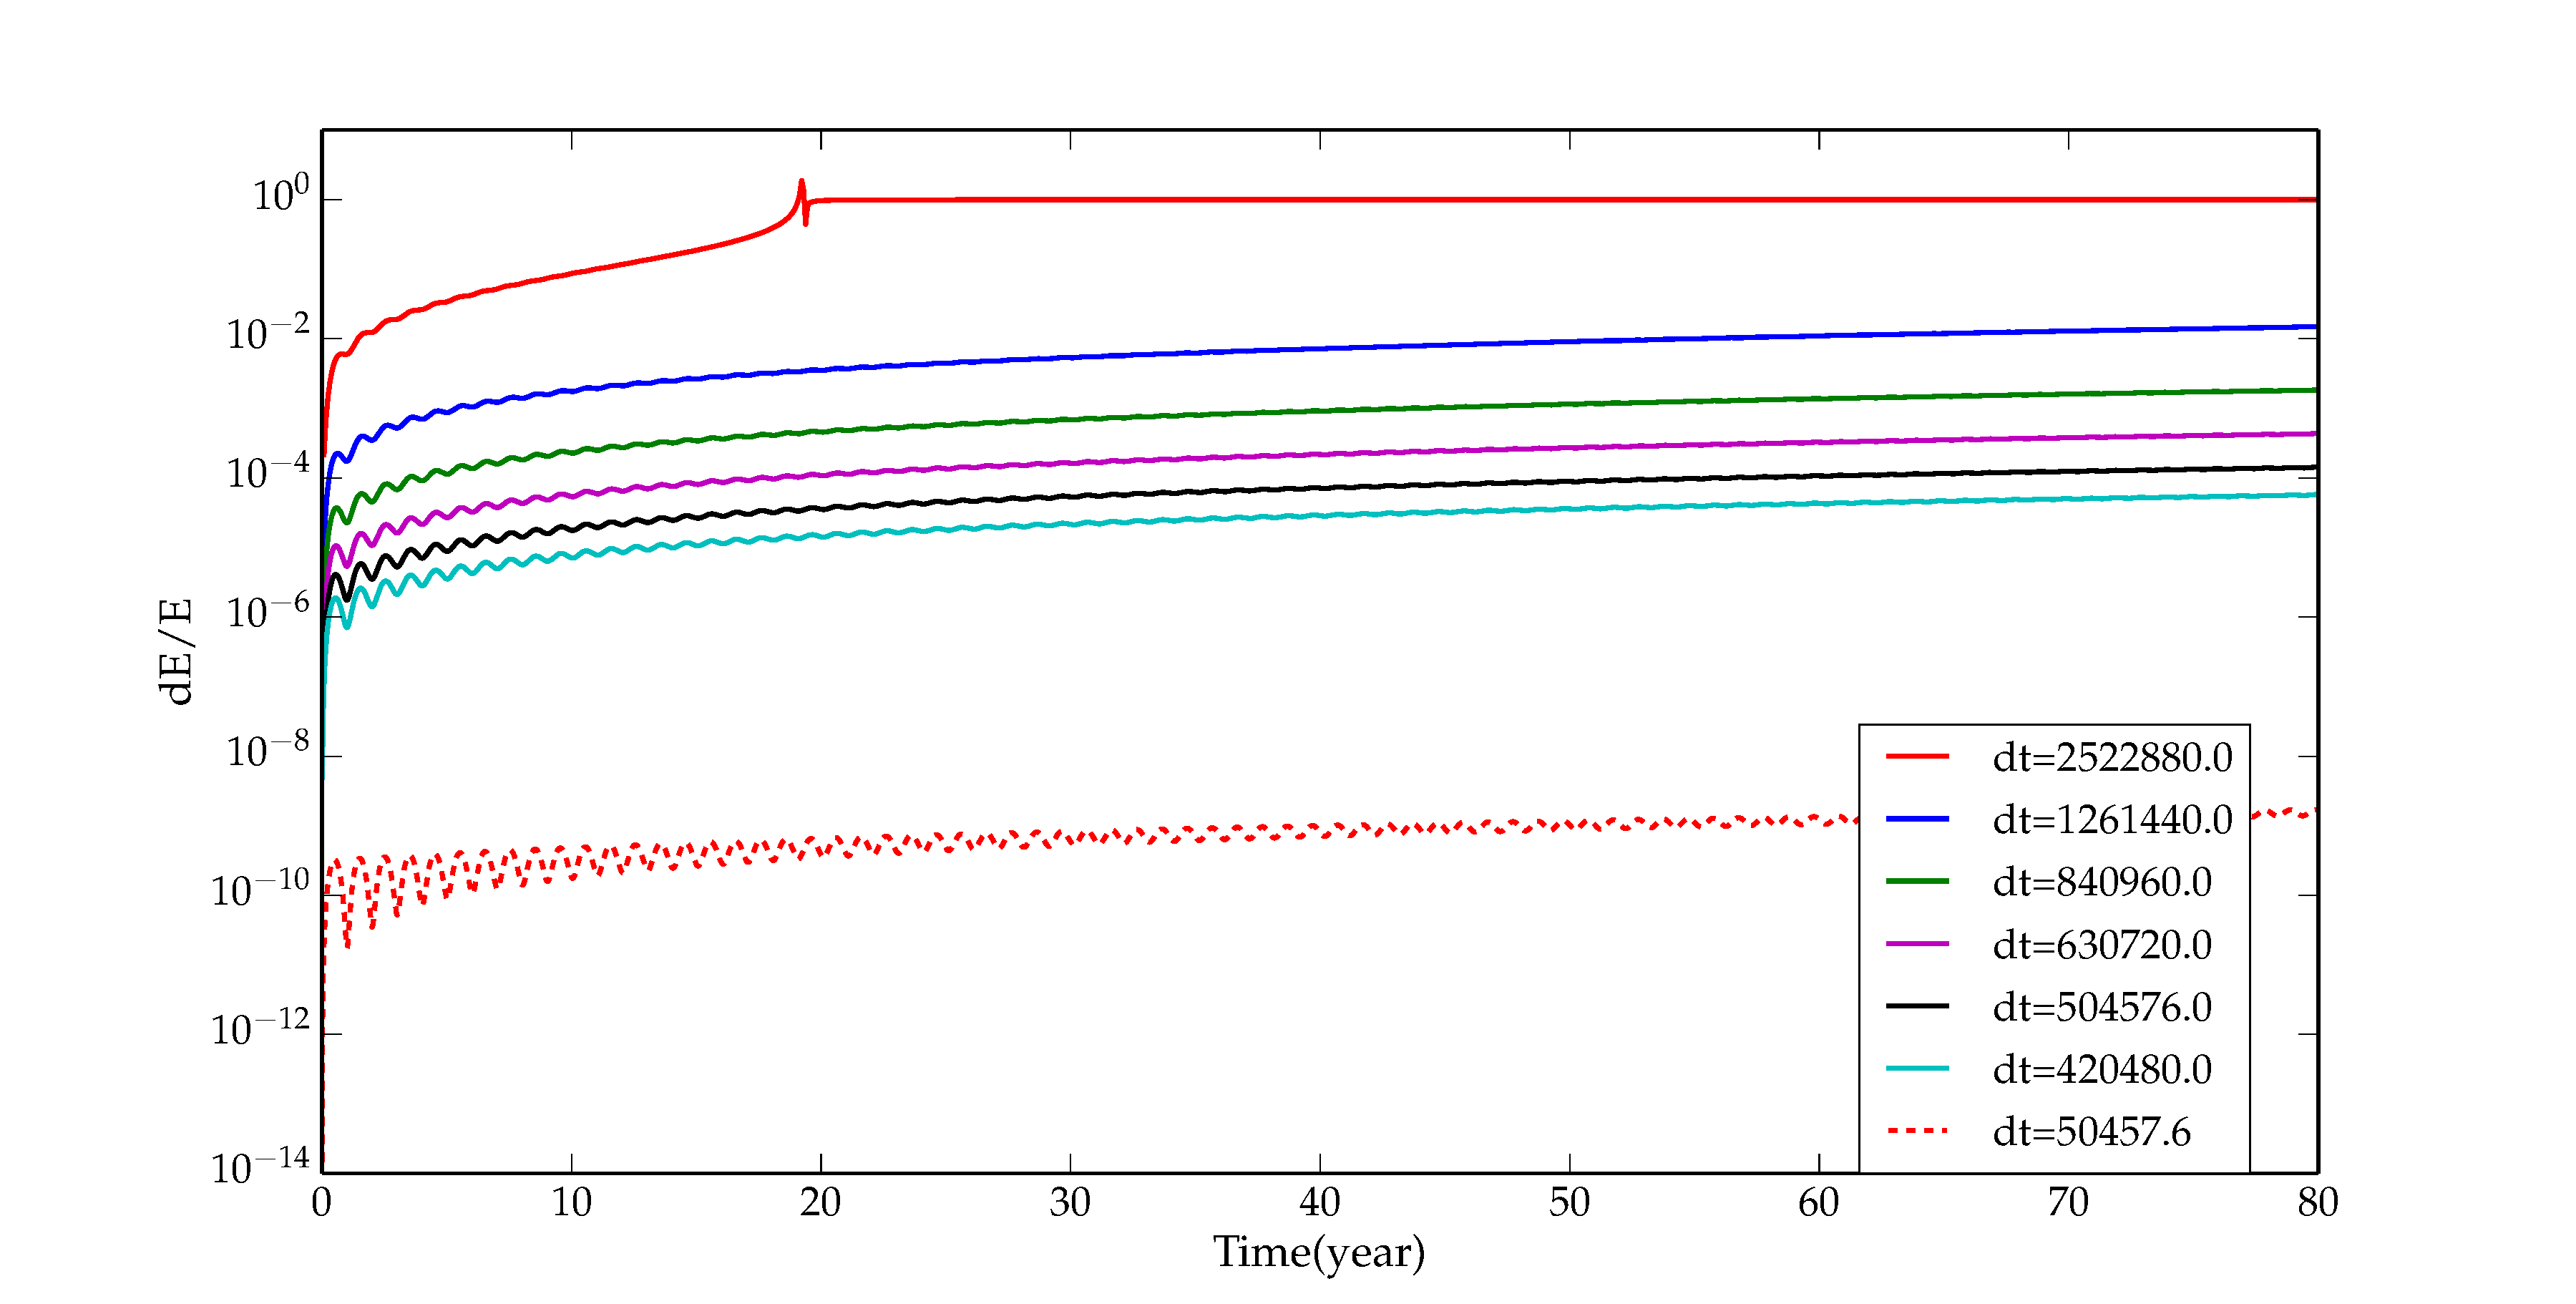
\includegraphics[height = 0.4\textheight]{Resolution}
	\caption{}
	\label{fig:Resolution}
\end{figure}

How does the resolution, or size of time step, affects the accumulated error of RK4 method? From figure \ref{fig:Resolution}, we can see that when the time step gets smaller, the accumulated error also gets smaller. At the worst resolution, the bold red line, the error accumulates up so much that it explodes at time around 20 years.

\begin{figure}[h!]
	\centering
	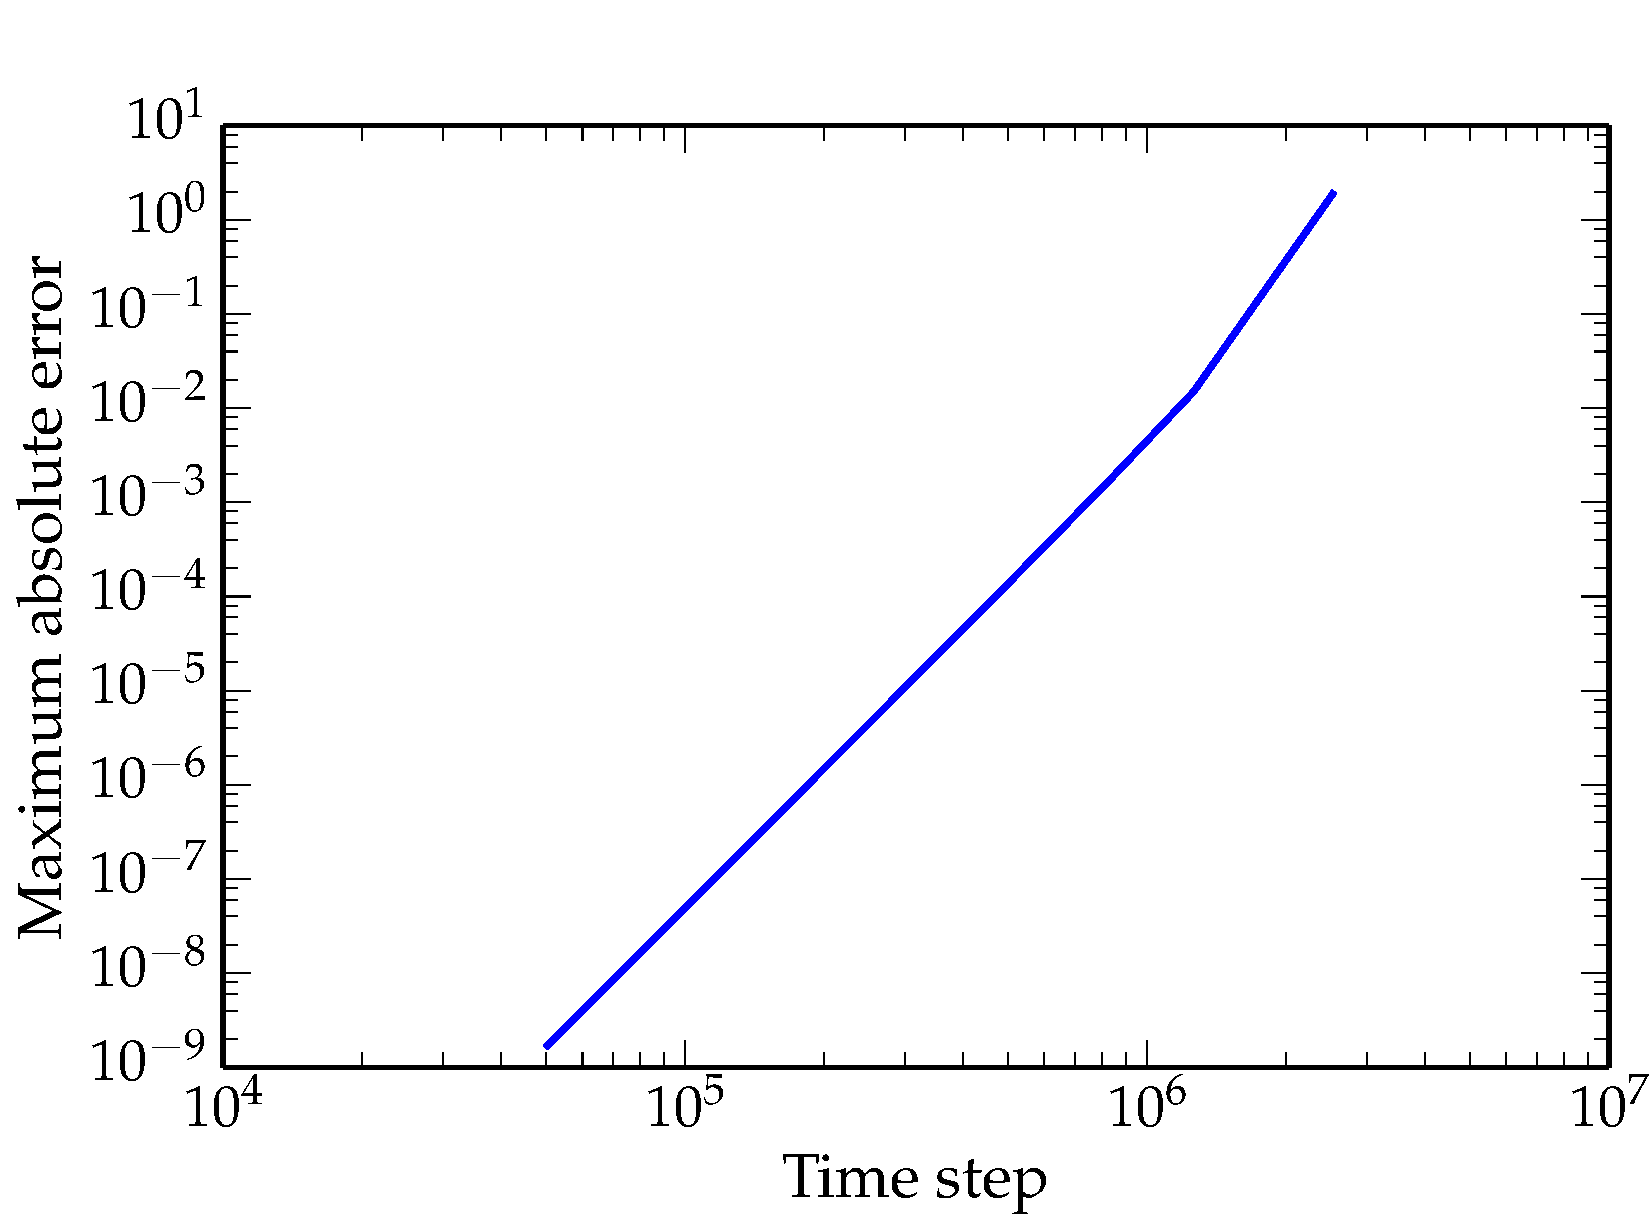
\includegraphics[width=0.5\textwidth]{Convergence}
	\caption{}
	\label{fig:Convergence}
\end{figure}

From figure \ref{fig:Resolution}, we can find the convergent rate of the RK4 method by plotting maximum error for each time step. Figure \ref{fig:Convergence} shows a line with slope of 4, which confirms RK4 being the 4th order error method.

\subsection{Eccentricity}

\begin{figure}[h!]
	\centering
	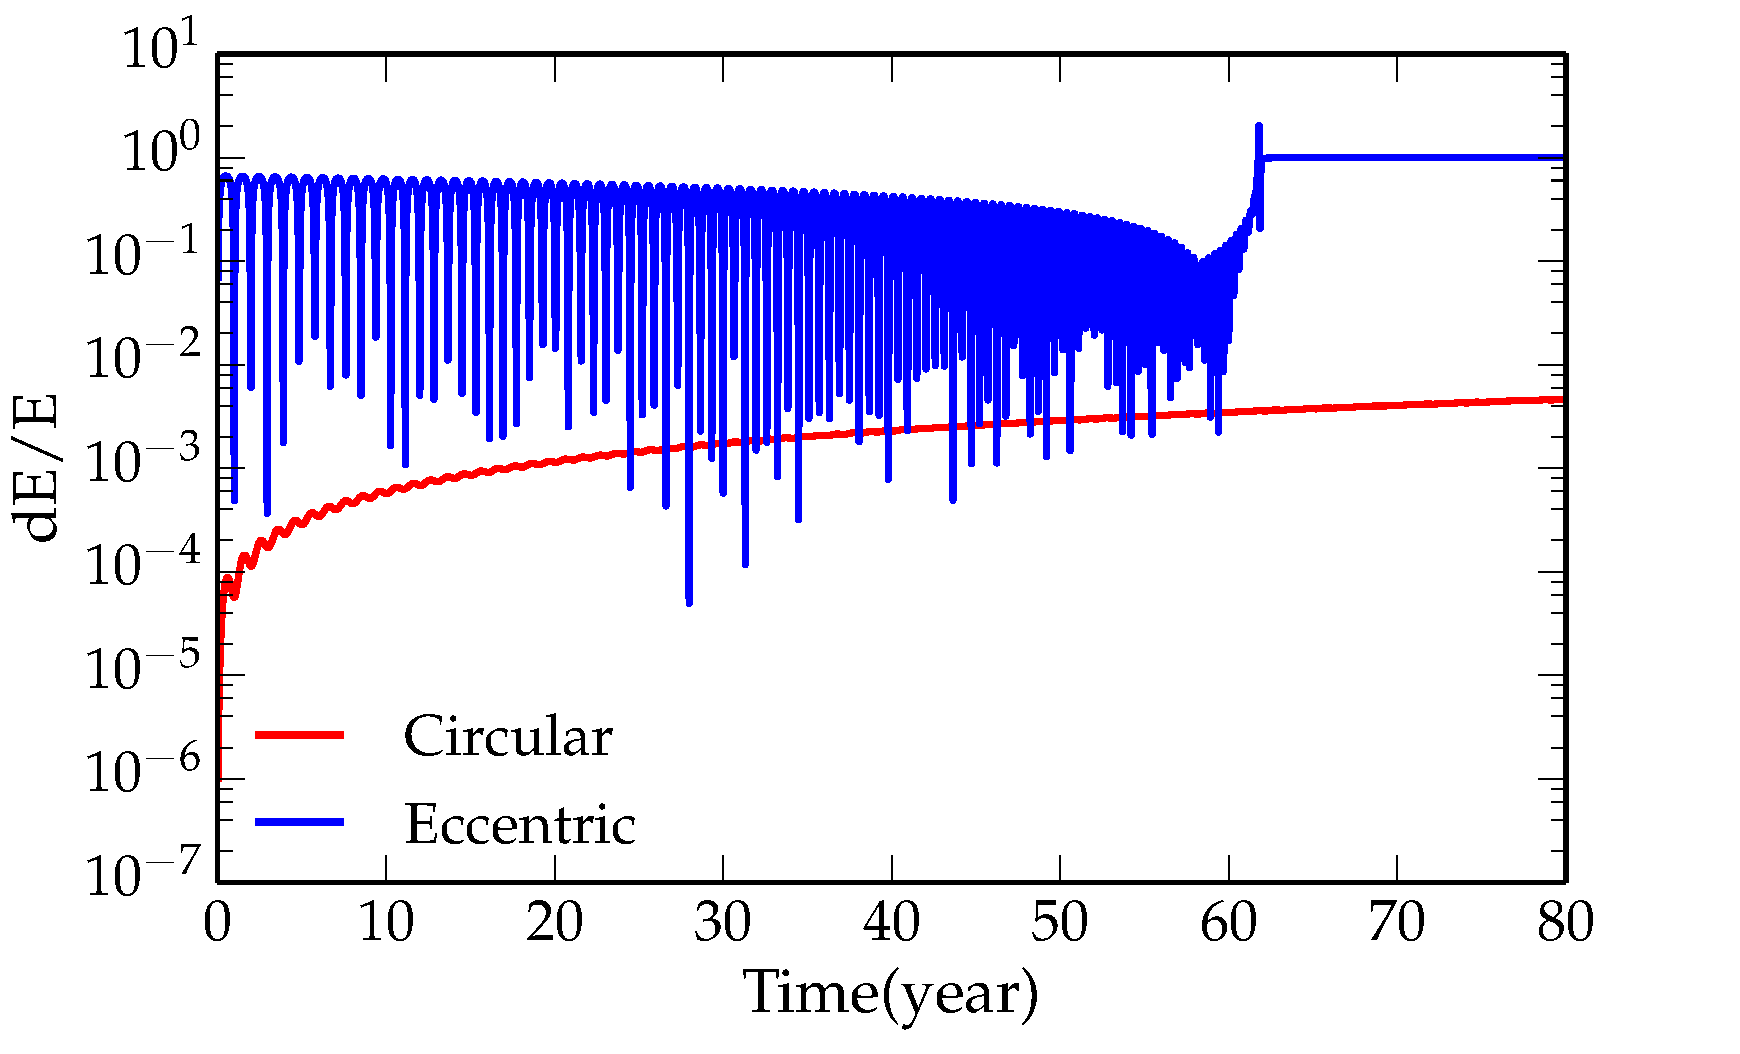
\includegraphics[width = 0.6\textwidth]{Eccentric_Error}
	\caption{}
	\label{fig:Eccentric_Error}
\end{figure}
	
Instead of being a circular orbit, I put the Earth at eccentricity of 0.5, which would be disastrous for humans. We compare the error of RK4 of circular and eccentric orbit. (Figure \ref{fig:Eccentric_Error}) Even though both of these orbits are integrated at the same size of time step, their errors are not the same. Even at the same resolution, error of the eccentric orbit blows up. Thus, for the rest of the project, we have to use higher resolution for eccentric orbit than for circular orbit.

\section{Adding the moon}

\begin{figure}[h!]
	\centering
	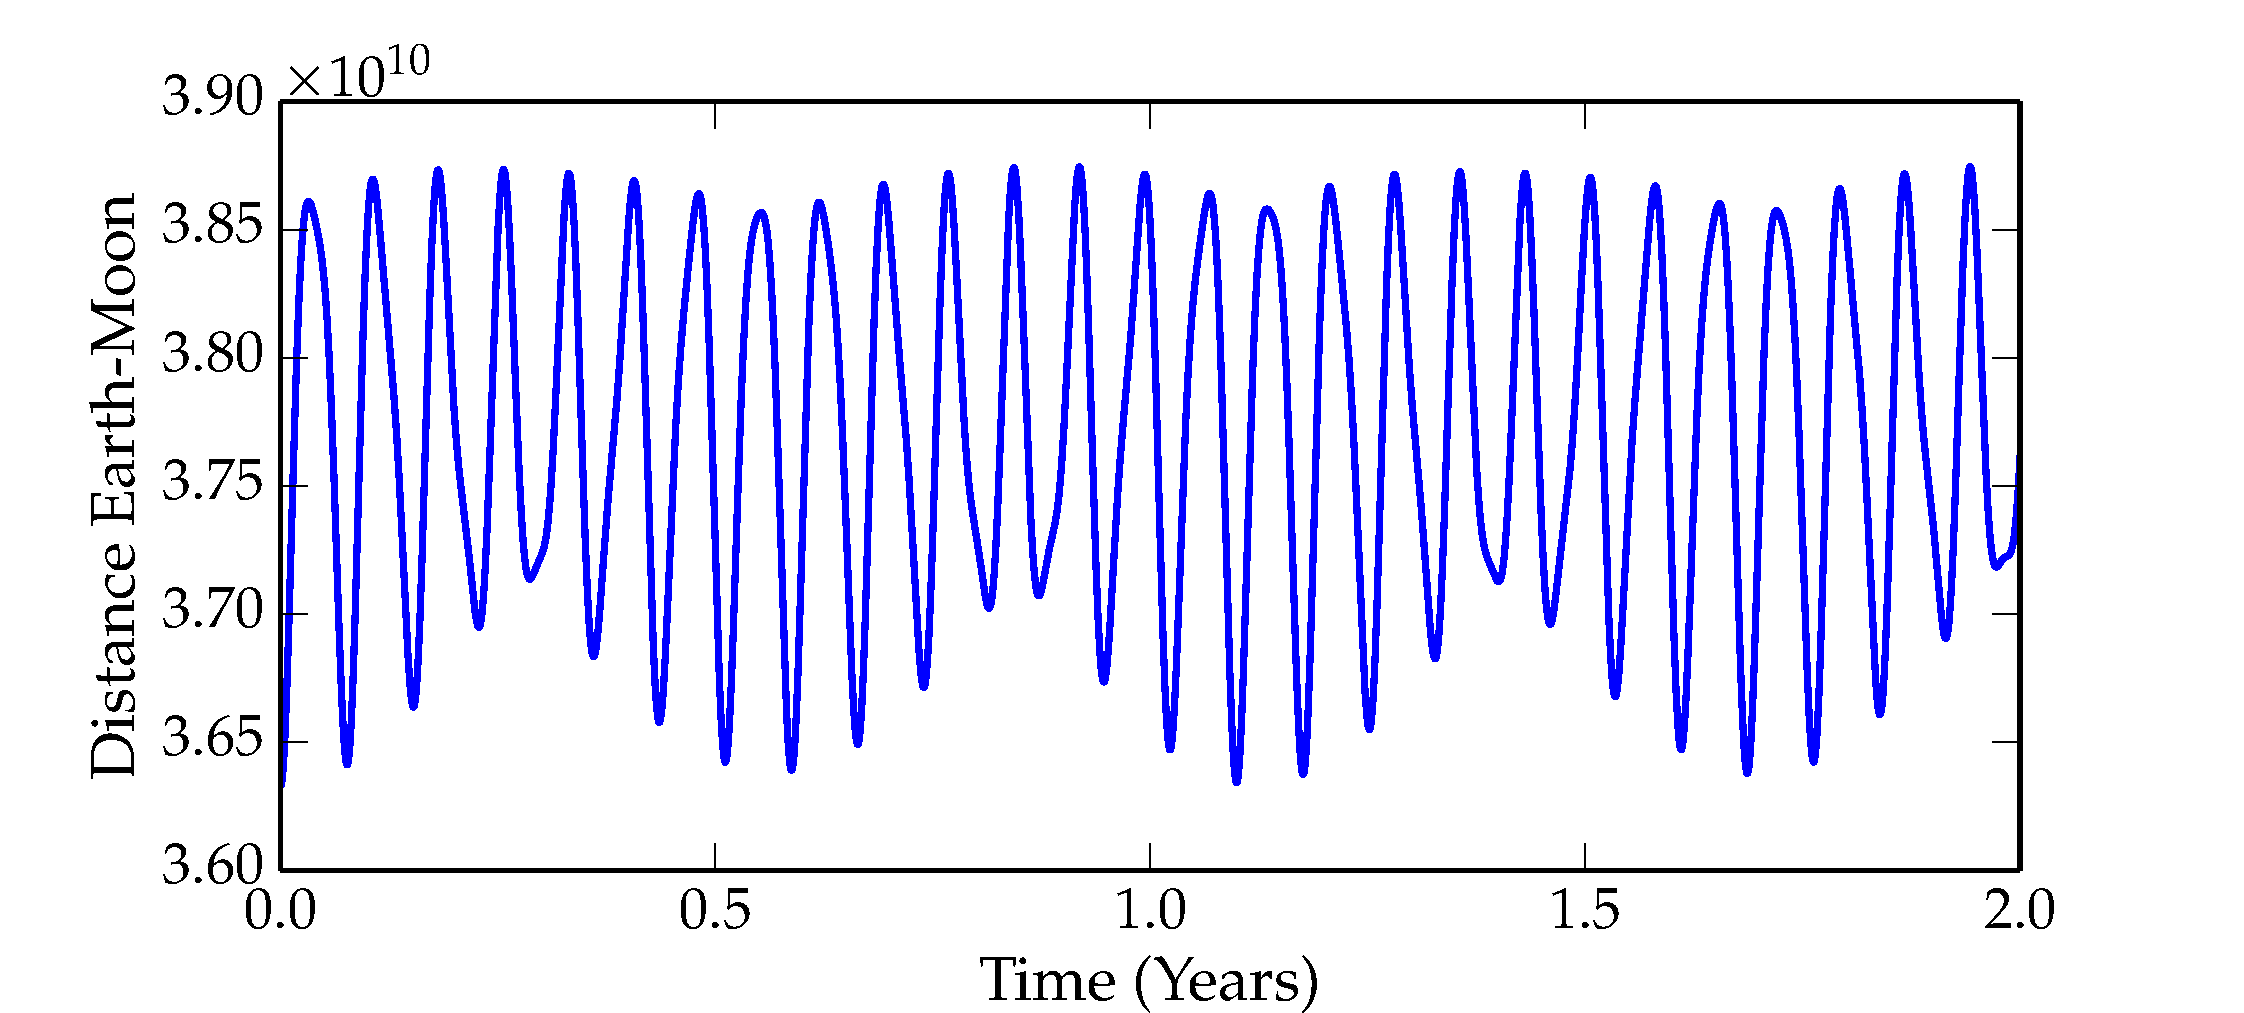
\includegraphics[height = 0.3\textheight]{Moon_Apsis}
	\caption{Distance between Earth and Moon over time. We can see that the apogee and perigee of each cycle is not the same. However, the changing in the apsis shows a sinusoidal features with a period of half a year.}
	\label{fig:Moon_Apsis}
\end{figure}

\begin{figure}[h!]
	\centering
	\includegraphics[width=0.5\textwidth]{Moon_Eccentricity}
	\caption{Based on data from figure \ref{fig:Moon_Apsis}, for each cycle, we use perigee and apogee to calculate the eccentricity of the moon orbit, assuming two-body system. On average, the eccentricity is about 0.027, which is about half of the real eccentricity of the moon.}
	\label{fig:Moon_Eccentricity}
\end{figure}

Using the same code as previous sections, we add moon into the system. Despite the moon has an inclination of 5 degree, we assume that the inclination angle to be 0 degree. Figure \ref{fig:Moon_Apsis} shows the distance between the Earth and Moon over time. We can see that the apsis of the moon orbit varies with a sinusoidal feature of period 0.5 year. This shows that the system is stable.

Based on the apsis of the system, by assuming the properties of two-body system, we can calculate the eccentricity of each orbit of the moon. Figure \ref{fig:Moon_Eccentricity} shows the eccentricity vs. time. To no surprise, it also shows sinusoidal feature. On average, the eccentricity is approximately 0.027, which is roughly half of the real value.

\section{Kozai Effect}

\begin{figure}[h!]
	\centering
	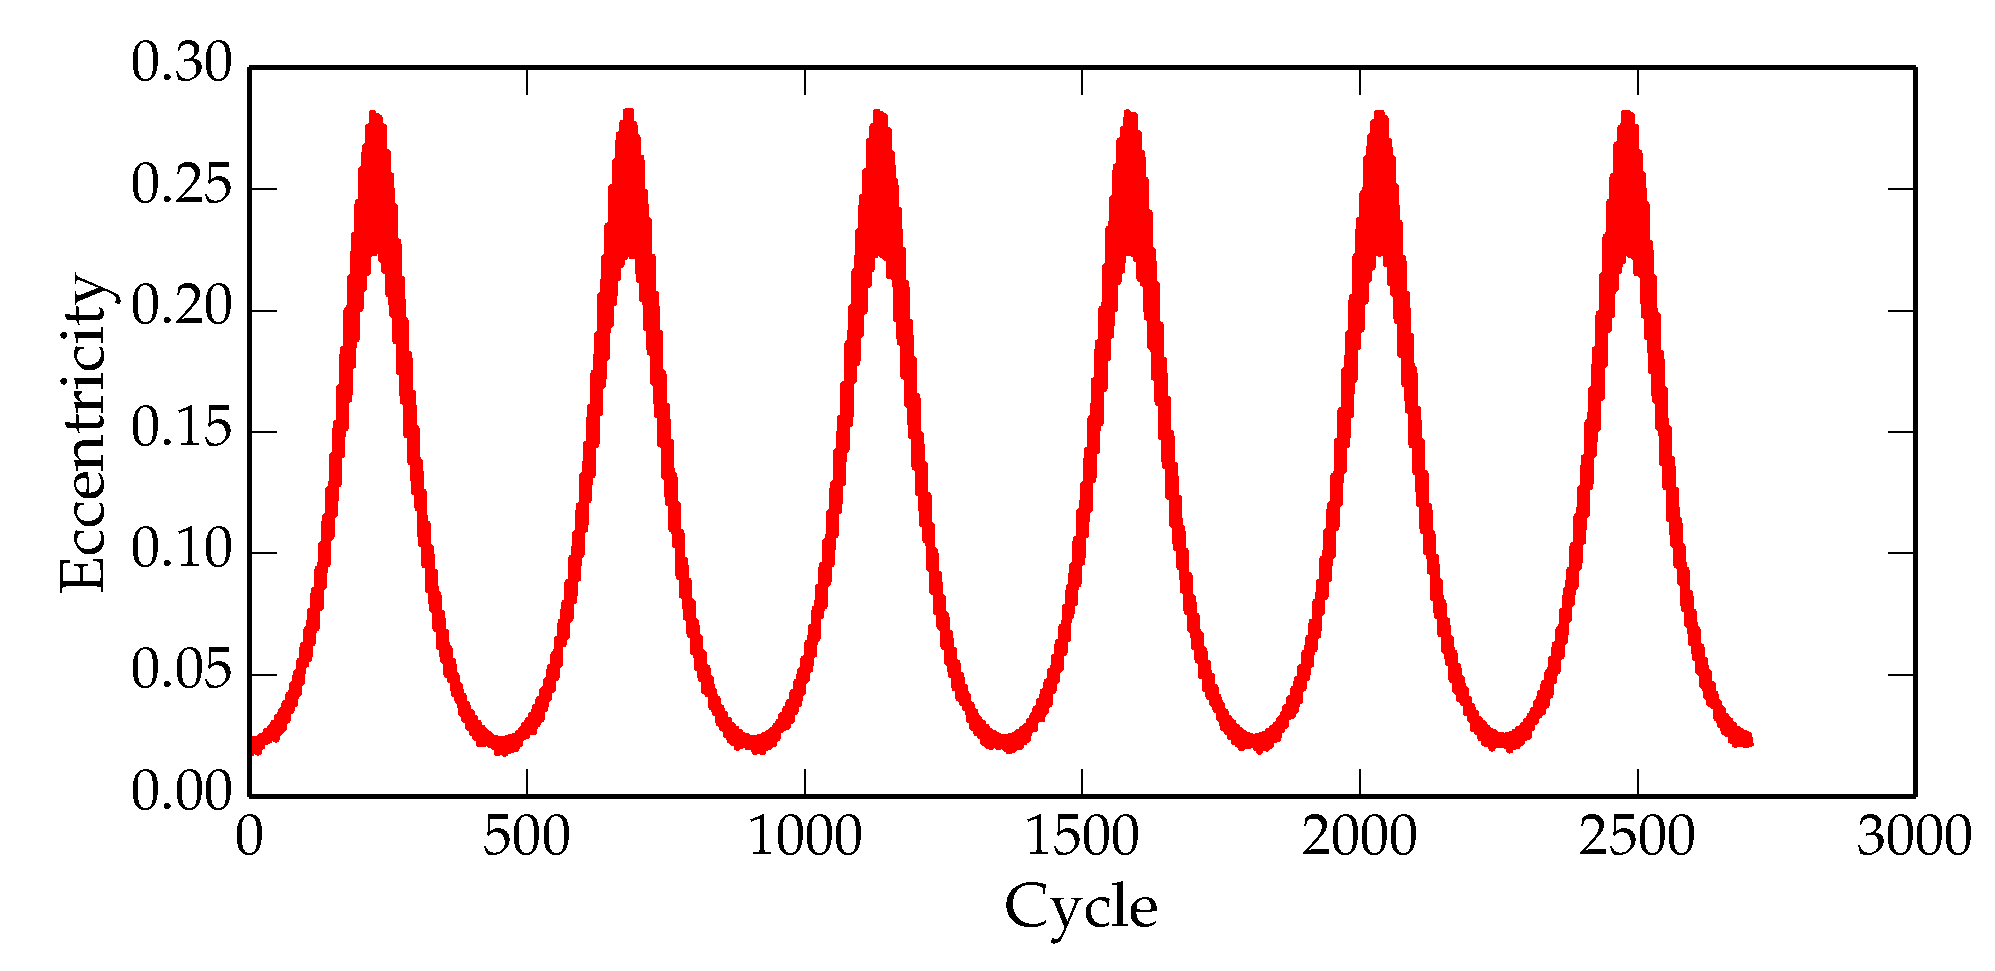
\includegraphics[height = 0.25\textheight]{Kozai_Ecc_Cycle}
	\caption{Plot the varying eccentricity of the moon, with initial inclination of 45 degree. With Kozai mechanism, losing inclination means gaining eccentricity, maximum eccentricity is reached when the inclination angle goes down to zero degree.}
	\label{fig:Kozai_Ecc_Cycle}
\end{figure}

\begin{figure}[h!]
	\centering
	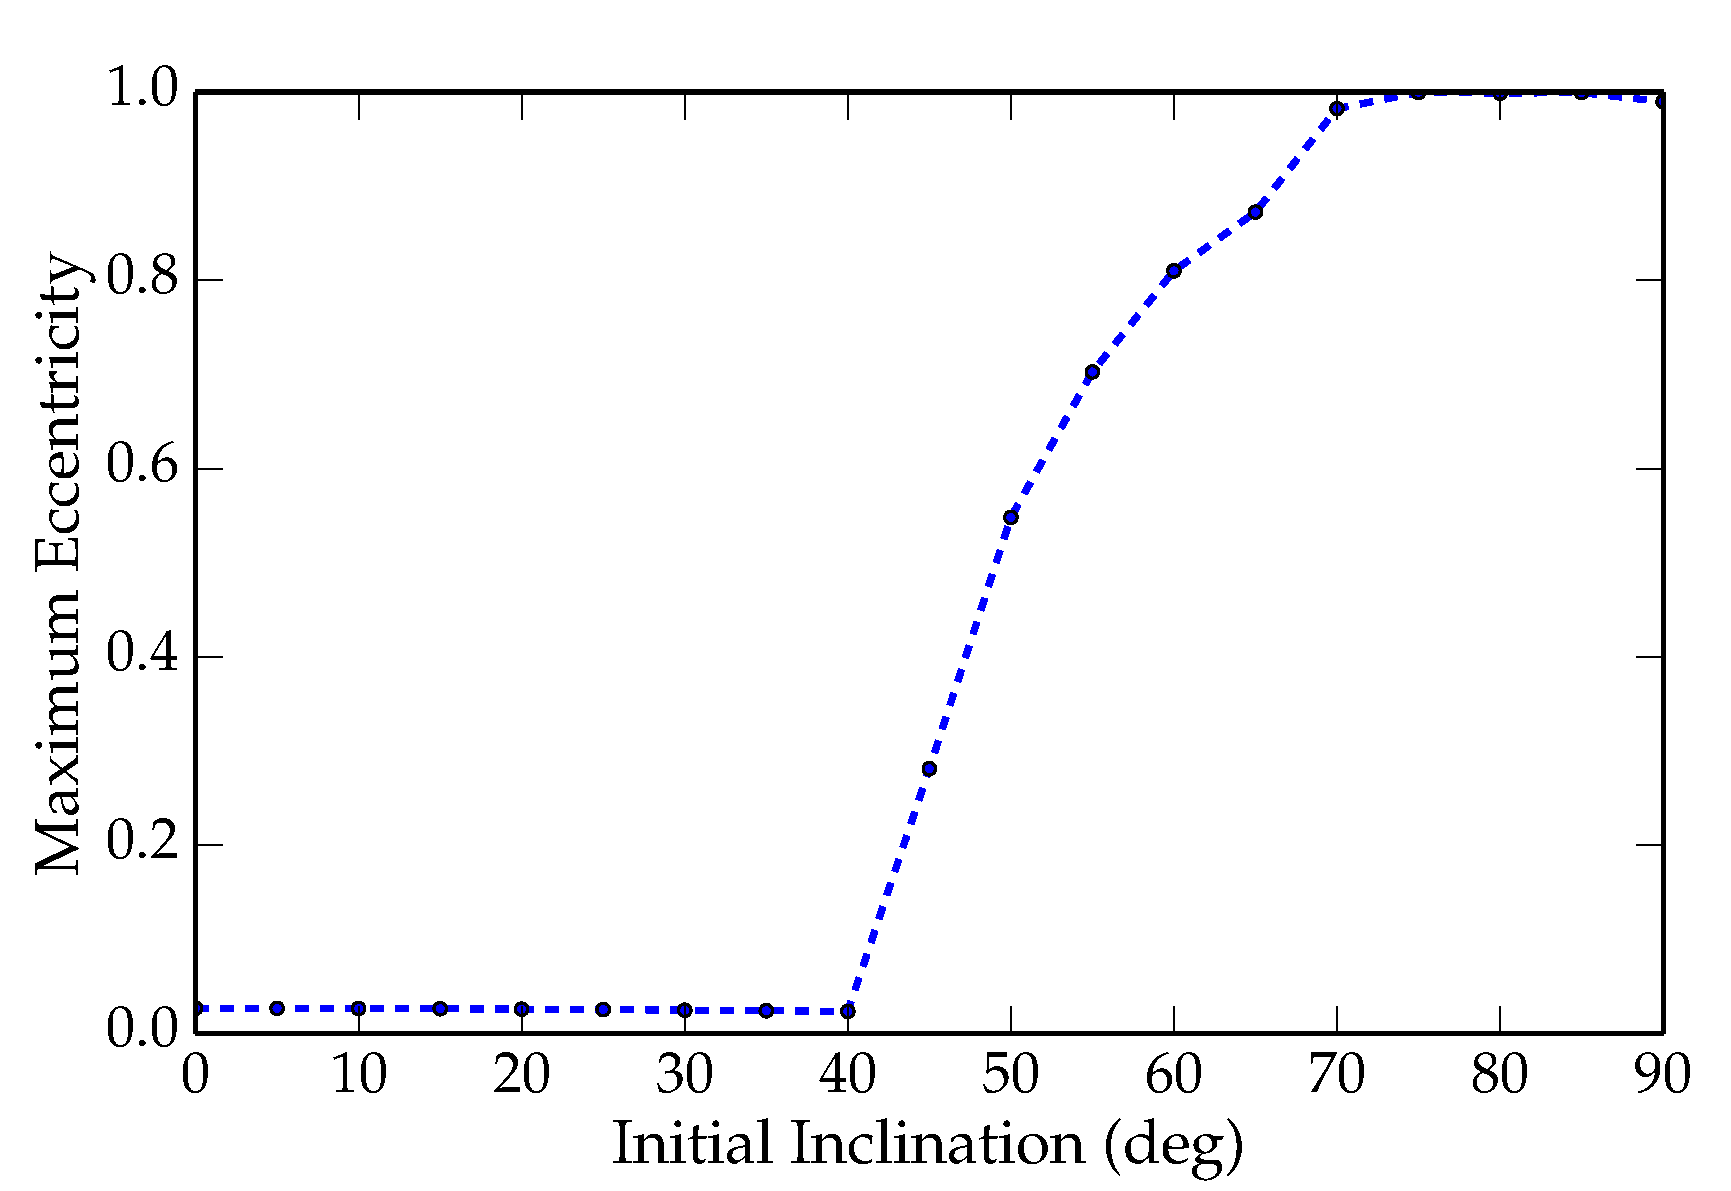
\includegraphics[width = 0.65\textwidth]{Max_Ecc}
	\caption{Varying the initial inclination angle. Then, plot the maximum eccentricity. If the initial inclination is less than roughly 40 degree, the eccentricity doesn't change much. However, if the initial inclination is larger than 40 degree, the orbit of the moon can get very elliptical.}
	\label{fig:Max_Ecc}
\end{figure}

Exploring the Kozai mechanism, which is a three-body phenomenon. A body with some initial inclination angle could trade off inclination for eccentricity. Initially, I put the moon at inclination angle of 45 degree to the Earth-Sun orbital plane. Using the code in previous sections, I monitor eccentricity of the moon orbit over time. (Figure \ref{fig:Kozai_Ecc_Cycle}) At cycle 0, the eccentricity is low, because off the initial condition. As time goes on, the eccentricity increases while the inclination angle decreases. Eccentricity reaches maximum when the inclination angle is 0 degree.

By varying the initial inclination angle, we get different maximum eccentricity. Figure \ref{fig:Max_Ecc} is similar to figure 6 of [Ford \emph{et al.} ApJ \textbf{535} 385 (2000)] If the initial inclination is less than roughly 40 degree, the eccentricity doesn't change much. However, if the initial inclination is larger than 40 degree, the orbit of the moon can get very elliptical. This is the same result found by Ford.

\end{document}

